\documentclass[10pt]{article}
\usepackage[ansinew]{inputenc}
\usepackage{makeidx,amsmath,amssymb,exscale,multicol,epsfig,graphics,verbatim,ulem}
\usepackage{epsfig,geometry,url,listings,subcaption}
\usepackage{boxedminipage}
\usepackage[T1]{fontenc}%required
\usepackage{textcomp}
\geometry{headsep=3ex,hscale=0.9}
\usepackage{hyperref}
\usepackage{color}
\hypersetup{pdftitle={GNUnet C Tutorial},
  pdfsubject={GNUnet},
  pdfauthor={Christian Grothoff <christian@grothoff.org>},
  pdfkeywords={p2p,search,gnunet,tutorial}
  %,pdfpagemode={FullScreen}
  }


\lstset{
language=bash,
basicstyle=\ttfamily,
upquote=true,
columns=fullflexible,
literate={*}{{\char42}}1
         {-}{{\char45}}1
}

\newcommand{\exercise}[1]{\noindent\begin{boxedminipage}{\textwidth}{\bf Exercise:} #1 \end{boxedminipage}}

\begin{document}

\lstset{ %
language=C,                     % choose the language of the code
basicstyle=\footnotesize,       % the size of the fonts that are used for the code
numbers=left,                   % where to put the line-numbers
numberstyle=\footnotesize,      % the size of the fonts that are used for the line-numbers
stepnumber=1,                   % the step between two line-numbers. If it is 1 each line will be numbered
numbersep=5pt,                  % how far the line-numbers are from the code
backgroundcolor=\color{white},  % choose the background color. You must add \usepackage{color}
showspaces=false,               % show spaces adding particular underscores
showstringspaces=false,         % underline spaces within strings
showtabs=false,                 % show tabs within strings adding particular underscores
frame=single,           % adds a frame around the code
tabsize=2,          % sets default tabsize to 2 spaces
captionpos=b,           % sets the caption-position to bottom
breaklines=true,        % sets automatic line breaking
breakatwhitespace=false,    % sets if automatic breaks should only happen at whitespace
escapeinside={\%*}{*)}          % if you want to add a comment within your code
}


\begin{center}
\large {A Tutorial for GNUnet 0.10.x (C version)}

Christian Grothoff $\qquad$ Bart Polot $\qquad$ Matthias Wachs

\today
\end{center}
This tutorials explains how to install GNUnet on a GNU/Linux system and gives an introduction on how
GNUnet can be used to develop a Peer-to-Peer application. Detailed installation instructions for
various operating systems and a detailed list of all dependencies can be found on our website at
\url{https://gnunet.org/installation}.

\textbf{Please read this tutorial carefully since every single step is
  important and do not hesitate to contact the GNUnet team if you have
  any questions or problems! Check here how to contact the GNUnet
  team: \url{https://gnunet.org/contact_information}}


\section{Installing GNUnet}

First of all you have to install a current version of GNUnet. You can download a
tarball of a stable version from GNU FTP mirrors or obtain the latest development
version from our Git repository.

Most of the time you should prefer to download the stable version since with the
latest development version things can be broken, functionality can be changed or tests
can fail. You should only use the development version if you know that you require a
certain feature or a certain issue has been fixed since the last release.

\subsection{Obtaining a stable version}

You can download the latest stable version of GNUnet from GNU FTP mirrors:
\begin{center}
\url{ftp://ftp.gnu.org/gnu/gnunet/gnunet-0.10.x.tar.gz}
\end{center}
You should also download the signature file and verify the integrity of the tarball.
\begin{center}
\url{ftp://ftp.gnu.org/gnu/gnunet/gnunet-0.10.x.tar.gz.sig}
\end{center}
To verify the signature you should first import the GPG key used to sign the tarball
\lstset{language=bash}
\begin{lstlisting}
$ gpg --keyserver keys.gnupg.net --recv-keys 48426C7E
\end{lstlisting}
And use this key to verify the tarball's signature
\lstset{language=bash}
\begin{lstlisting}
$ gpg --verify gnunet-0.10.x.tar.gz.sig gnunet-0.10.x.tar.gz
\end{lstlisting}
After successfully verifying the integrity you can extract the tarball using
\lstset{language=bash}
\begin{lstlisting}
$ tar xvzf gnunet-0.10.x.tar.gz
$ mv gnunet-0.10.x gnunet		# we will use the directory "gnunet" in the remainder of this document
$ cd gnunet
\end{lstlisting}

However, please note that stable versions can be very outdated, as a developer
you are strongly encouraged to use the version from \url{https://gnunet.org/git/}.

\subsection{Installing Build Tool Chain and Dependencies}

To successfully compile GNUnet you need the tools to build GNUnet and the required dependencies.
Please have a look at \url{https://gnunet.org/dependencies} for a list of required dependencies
and \url{https://gnunet.org/generic_installation} for specific instructions for your operating system.

Please check the notes at the end of the configure process about required dependencies.

For GNUnet bootstrapping support and the http(s) plugin you should install \texttt{libgnurl}.
For the filesharing service you should install at least one of the datastore backends \texttt{mysql},
\texttt{sqlite} or \texttt{postgresql}.

\subsection{Obtaining the latest version from Git}

The latest development version can obtained from our Git repository. To obtain
the code you need Git installed and checkout the repository using:
\lstset{language=bash}
\begin{lstlisting}
$ git clone https://gnunet.org/git/gnunet
\end{lstlisting}
After cloning the repository you have to execute
\lstset{language=bash}
\begin{lstlisting}
$ cd gnunet
$ ./bootstrap
\end{lstlisting}

The remainder of this tutorial assumes that you have Git Master checked out.


\subsection{Compiling and Installing GNUnet}

First, you need to install at least {\tt libgnupgerror} version
1.27\footnote{\url{ftp://ftp.gnupg.org/gcrypt/libgpg-error/libgpg-error-1.27.tar.bz2}}
and {\tt libgcrypt} version
1.7.6\footnote{\url{ftp://ftp.gnupg.org/gcrypt/libgcrypt/libgcrypt-1.7.6.tar.bz2}}.

\lstset{language=bash}
\begin{lstlisting}
$ wget ftp://ftp.gnupg.org/gcrypt/libgpg-error/libgpg-error-1.27.tar.bz2
$ tar xf libgpg-error-1.27.tar.bz2
$ cd libgpg-error-1.27
$ ./configure
$ sudo make install
$ cd ..
\end{lstlisting}

\lstset{language=bash}
\begin{lstlisting}
$ wget ftp://ftp.gnupg.org/gcrypt/libgcrypt/libgcrypt-1.7.6.tar.bz2
$ tar xf libgcrypt-1.7.6.tar.bz2
$ cd libgcrypt-1.7.6
$ ./configure
$ sudo make install
$ cd ..
\end{lstlisting}

\label{sub:install}
Assuming all dependencies are installed, the following commands will
compile and install GNUnet in your home directory. You can specify the
directory where GNUnet will be installed by changing the
\lstinline|--prefix| value when calling \lstinline|./configure|.  If
you do not specifiy a prefix, GNUnet is installed in the directory
\lstinline|/usr/local|. When developing new applications you may want
to enable verbose logging by adding
\lstinline|--enable-logging=verbose|:

\lstset{language=bash}
\begin{lstlisting}
$ ./configure --prefix=$PREFIX --enable-logging
$ make
$ make install
\end{lstlisting}

After installing GNUnet you have to add your GNUnet installation to your path
environmental variable. In addition you have to create the \lstinline|.config|
directory in your home directory where GNUnet stores its data and an empty
GNUnet configuration file:

\lstset{language=bash}
\begin{lstlisting}
$ export PATH=$PATH:$PREFIX/bin
$ echo export PATH=$PREFIX/bin:\\$PATH >> ~/.bashrc
$ mkdir ~/.config/
$ touch ~/.config/gnunet.conf
\end{lstlisting}
% $

\subsection{Common Issues - Check your GNUnet installation}

You should check your installation to ensure that installing GNUnet
was successful up to this point. You should be able to access GNUnet's
binaries and run GNUnet's self check.
\lstset{language=bash}
\begin{lstlisting}
$ which gnunet-arm
\end{lstlisting}
should return \lstinline|$PREFIX/bin/gnunet-arm|. It should be
located in your GNUnet installation and the output should not be
empty. If you see an output like:
\lstset{language=bash}
\begin{lstlisting}
$ which gnunet-arm
$
\end{lstlisting}
check your {\tt PATH} variable to ensure GNUnet's {\tt bin} directory is included.

GNUnet provides tests for all of its subcomponents. Run
\lstset{language=bash}
\begin{lstlisting}
$ make check
\end{lstlisting}
to execute tests for all components. {\tt make check} traverses all subdirectories in {\tt src}.
For every subdirectory you should get a message like this:

\begin{verbatim}
make[2]: Entering directory `/home/$USER/gnunet/contrib'
PASS: test_gnunet_prefix
=============
1 test passed
=============
\end{verbatim}


\section{Background: GNUnet Architecture}

GNUnet is organized in layers and services. Each service is composed of a
main service implementation and a client library for other programs to use
the service's functionality, described by an API. This approach is shown in
figure~\ref{fig:service}. Some services provide an additional command line
tool to enable the user to interact with the service.

Very often it is other GNUnet services that will use these APIs to build the
higher layers of GNUnet on top of the lower ones. Each layer expands or extends
the functionality of the service below (for instance, to build a mesh on top of
a DHT). See figure ~\ref{fig:interaction} for an illustration of this approach.

\begin{figure}[!h]
  \begin{center}
%  \begin{subfigure}
        \begin{subfigure}[b]{0.3\textwidth}
                \centering
                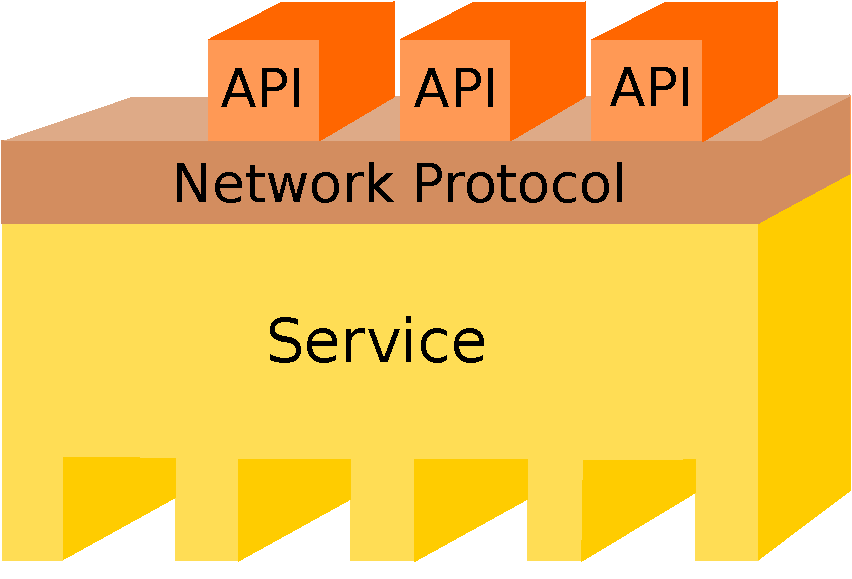
\includegraphics[width=\textwidth]{figs/Service.pdf}
                \caption{Service with API and network protocol}
                \label{fig:service}
        \end{subfigure}
        ~~~~~~~~~~
        \begin{subfigure}[b]{0.3\textwidth}
                \centering
                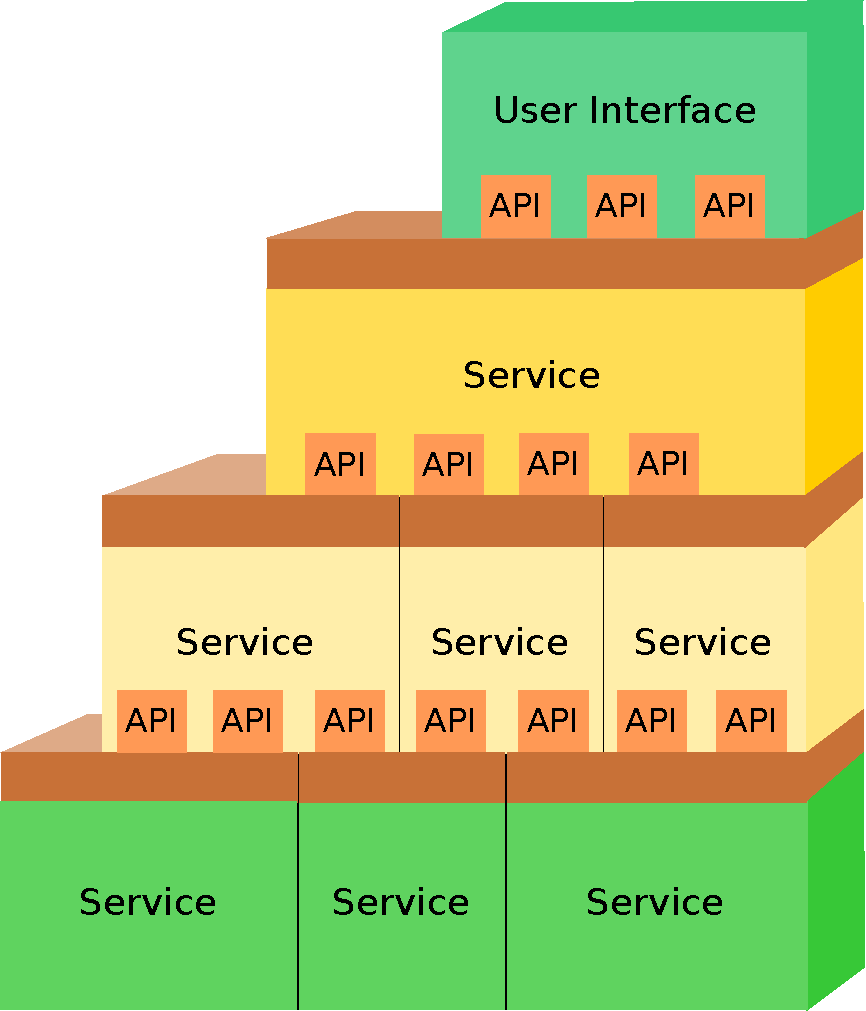
\includegraphics[width=\textwidth]{figs/System.pdf}
                \caption{Service interaction}
                \label{fig:interaction}
        \end{subfigure}
  \end{center}
  \caption{GNUnet's layered system architecture}
\end{figure}

The main service implementation runs as a standalone process in the operating
system and the client code runs as part of the client program, so crashes of a
client do not affect the service process or other clients. The service and the
clients communicate via a message protocol to be defined and implemented by
the programmer.


\section{First Steps with GNUnet}

\subsection{Configure your peer}

First of all we need to configure your peer. Each peer is started with a configuration containing settings for GNUnet itself and its services. This configuration is based on the default configuration shipped with GNUnet and can be modified. The default configuration is located in the {\tt \$PREFIX/share/gnunet/config.d} directory. When starting a peer, you can specify a customized configuration using the the {\tt$-c$} command line switch when starting the ARM service and all other services. When using a modified configuration the default values are loaded and only values specified in the configuration file will replace the default values.

Since we want to start additional peers later, we need
some modifications from the default configuration. We need to create a separate service home and a file containing our modifications for this peer:
\lstset{language=bash}
\begin{lstlisting}
$ mkdir ~/gnunet1/
$ touch peer1.conf
\end{lstlisting}

Now add the following lines to peer1.conf to use this directory. For
simplified usage we want to prevent the peer to connect to the GNUnet
network since this could lead to confusing output. This modifications
will replace the default settings:
\begin{verbatim}
[PATHS]
GNUNET_HOME = ~/gnunet1/		# Use this directory to store GNUnet data
[hostlist]
SERVERS =				# prevent bootstrapping
\end{verbatim}


\subsection{Start a peer}
Each GNUnet instance (called peer) has an identity (\textit{peer ID}) based on a
cryptographic public private key pair. The peer ID is the printable hash of the
public key.

GNUnet services are controlled by a master service the so called \textit{Automatic Restart Manager} (ARM).
ARM starts, stops and even restarts services automatically or on demand when a client connects.
You interact with the ARM service using the \lstinline|gnunet-arm| tool.
GNUnet can then be started with \lstinline|gnunet-arm -s| and stopped with
\lstinline|gnunet-arm -e|.  An additional service not automatically started
can be started using \lstinline|gnunet-arm -i <service name>| and stopped
using \lstinline|gnunet-arm -k <servicename>|.

Once you have started your peer, you can use many other GNUnet commands
to interact with it.  For example, you can run:
\lstset{language=bash}
\begin{lstlisting}
$ gnunet-peerinfo -s
\end{lstlisting}
to obtain the public key of your peer.
You should see an output containing the peer ID similar to:
\lstset{language=bash}
\begin{lstlisting}
I am peer `0PA02UVRKQTS2C .. JL5Q78F6H0B1ACPV1CJI59MEQUMQCC5G'.
\end{lstlisting}


\subsection{Monitor a peer}

In this section, we will monitor the behaviour of our peer's DHT service with respect to a
specific key. First we will start GNUnet and then start the DHT service and use the DHT monitor tool
to monitor the PUT and GET commands we issue ussing the \lstinline|gnunet-dht-put| and
\lstinline|gnunet-dht-get| commands. Using the ``monitor'' line given below, you can observe the behavior of
your own peer's DHT with respect to the specified KEY:

\lstset{language=bash}
\begin{lstlisting}
$ gnunet-arm -c ~/peer1.conf -s			# start gnunet with all default services
$ gnunet-arm -c ~/peer1.conf -i dht		# start DHT service
$ cd ~/gnunet/src/dht;
$ ./gnunet-dht-monitor -c ~/peer1.conf -k KEY
\end{lstlisting}
Now open a separate terminal and change again to the \lstinline|gnunet/src/dht| directory:
\lstset{language=bash}
\begin{lstlisting}
$ cd ~/gnunet/src/dht
$ ./gnunet-dht-put -c ~/peer1.conf -k KEY -d VALUE		# put VALUE under KEY in the DHT
$ ./gnunet/src/dht/gnunet-dht-get -c ~/peer1.conf -k KEY	# get key KEY from the DHT
$ gnunet-statistics -c ~/peer1.conf		# print statistics about current GNUnet state
$ gnunet-statistics -c ~/peer1.conf -s dht	# print statistics about DHT service
\end{lstlisting}
% $


\subsection{Starting Two Peers by Hand}

\subsubsection{Setup a second peer}
We will now start a second peer on your machine.
For the second peer, you will need to manually create a modified
configuration file to avoid conflicts with ports and directories.
A peers configuration file is by default located in {\tt ~/.gnunet/gnunet.conf}.
This file is typically very short or even empty as only the differences to the
defaults need to be specified.  The defaults are located in
many files in the {\tt \$PREFIX/share/gnunet/config.d} directory.

To configure the second peer, use the files {\tt
  \$PREFIX/share/gnunet/config.d} as a template for your main
configuration file:
%
\lstset{language=bash}
\lstset{language=bash}
\begin{lstlisting}
$ cat $PREFIX/share/gnunet/config.d/*.conf > peer2.conf
\end{lstlisting}
Now you have to edit {\tt peer2.conf} and change:
\begin{itemize}
  \itemsep0em
  \item{\texttt{SERVICEHOME} under \texttt{PATHS}}
  \item{Every (uncommented) value for ``\texttt{PORT}'' (add 10000) in any
        section (the option may be commented out if \texttt{PORT} is
        prefixed by "\#", in this case, UNIX domain sockets are used
        and the PORT option does not need to be touched) }
  \item{Every value for ``\texttt{UNIXPATH}'' in any section (e.g. by adding a "-p2" suffix)}
\end{itemize}
to a fresh, unique value.  Make sure that the \texttt{PORT} numbers stay
below 65536.  From now on, whenever you interact with the second
peer, you need to specify {\tt -c peer2.conf} as an additional
command line argument.

Now, generate the 2nd peer's private key:

\lstset{language=bash}
\begin{lstlisting}
$ gnunet-peerinfo -s -c peer2.conf
\end{lstlisting}
% $

This may take a while, generate entropy using your keyboard or mouse
as needed.  Also, make sure the output is different from the {\tt
  gnunet-peerinfo} output for the first peer (otherwise you made an
error in the configuration).

\subsubsection{Start the second peer and connect the peers}

Then, you can start a second peer using:
\lstset{language=bash}
\begin{lstlisting}
$ gnunet-arm -c peer2.conf -s
$ gnunet-arm -c peer2.conf -i dht
$ ~/gnunet/src/dht/gnunet-dht-put -c peer2.conf -k KEY -d VALUE
$ ~/gnunet/src/dht/gnunet-dht-get -c peer2.conf -k KEY
\end{lstlisting}
If you want the two peers to connect, you have multiple options:
\begin{itemize}
\itemsep0em
  \item UDP neighbour discovery (automatic)
  \item Setup a bootstrap server
  \item Connect manually
\end{itemize}
To setup peer 1 as bootstrapping server change the configuration of
the first one to be a hostlist server by adding the following lines to
\texttt{peer1.conf} to enable bootstrapping server:
 \begin{verbatim}
[hostlist]
OPTIONS = -p
\end{verbatim}

Then change {\tt peer2.conf} and replace the ``\texttt{SERVERS}'' line in the ``\texttt{[hostlist]}'' section with
``\texttt{http://localhost:8080/}''.  Restart both peers using:
\begin{lstlisting}
$ gnunet-arm -c peer1.conf -e		# stop first peer
$ gnunet-arm -c peer1.conf -s		# start first peer
$ gnunet-arm -c peer2.conf -s		# start second peer
\end{lstlisting}

Note that if you start your peers without changing these settings, they
will use the ``global'' hostlist servers of the GNUnet P2P network and
likely connect to those peers.  At that point, debugging might become
tricky as you're going to be connected to many more peers and would
likely observe traffic and behaviors that are not explicitly controlled
by you.

\subsubsection{How to connect manually}

If you want to use the \texttt{peerinfo} tool to connect your peers, you should:
\begin{itemize}
\itemsep0em
 \item{Set {\tt FORCESTART = NO} in section {\tt hostlist} (to not connect to the global GNUnet)}
 \item{Start both peers running {\tt gnunet-arm -c peer1.conf -s} and {\tt gnunet-arm -c peer2.conf -s}}
 \item{Get \texttt{HELLO} message of the first peer running {\tt gnunet-peerinfo -c peer1.conf -g}}
 \item{Give the output to the second peer by running {\tt gnunet-peerinfo -c peer2.conf -p '<output>'}}
\end{itemize}

Check that they are connected using {\tt gnunet-core -c peer1.conf}, which should give you the other peer's
peer identity:
\lstset{language=bash}
\begin{lstlisting}
$ gnunet-core -c peer1.conf
Peer `9TVUCS8P5A7ILLBGO6 [...shortened...] 1KNBJ4NGCHP3JPVULDG'
\end{lstlisting}

\subsection{Starting Peers Using the Testbed Service}

GNUnet's testbed service is used for testing scenarios where a number of peers
are to be started.  The testbed can manage peers on a single host or on multiple
hosts in a distributed fashion.  On a single affordable computer, it should be
possible to run around tens of peers without drastically increasing the load on the
system.

The testbed service can be access through its API
\texttt{include/gnunet\_testbed\_service.h}.  The API provides many routines for
managing a group of peers.  It also provides a helper function
\texttt{GNUNET\_TESTBED\_test\_run()} to quickly setup a minimalistic testing
environment on a single host.

This function takes a configuration file which will be used as a template
configuration for the peers.  The testbed takes care of modifying relevant
options in the peers' configuration such as SERVICEHOME, PORT, UNIXPATH to
unique values so that peers run without running into conflicts.  It also checks
and assigns the ports in configurations only if they are free.

Additionally, the testbed service also reads its options from the same
configuration file.  Various available options and details about them can be
found in the testbed default configuration file \texttt{src/testbed/testbed.conf}.

With the testbed API, a sample test case can be structured as follows:
% <lynX> Is there a way to pick a more readable font for this include?
\lstset{language=C}
\lstinputlisting{testbed_test.c}
The source code for the above listing can be found at
\url{https://gnunet.org/git/gnunet.git/tree/doc/testbed_test.c}
or in the {\tt doc/} folder of your repository check-out.
After installing GNUnet, the above source code can be compiled as:
\lstset{language=bash}
\begin{lstlisting}
$ export CPPFLAGS="-I/path/to/gnunet/headers"
$ export LDFLAGS="-L/path/to/gnunet/libraries"
$ gcc $CPPFLAGS $LDFLAGS -o testbed-test testbed_test.c  -lgnunettestbed -lgnunetdht -lgnunetutil
\end{lstlisting}
The \texttt{CPPFLAGS} and \texttt{LDFLAGS} are necessary if GNUnet is installed
into a different directory other than \texttt{/usr/local}.

All of testbed API's peer management functions treat management actions as
operations and return operation handles.  It is expected that the operations
begin immediately, but they may get delayed (to balance out load on the system).
The program using the API then has to take care of marking the operation as
``done'' so that its associated resources can be freed immediately and other
waiting operations can be executed.  Operations will be canceled if they are
marked as ``done'' before their completion.

An operation is treated as completed when it succeeds or fails.  Completion of
an operation is either conveyed as events through \textit{controller event
  callback} or through respective operation completion callbacks.  In functions
which support completion notification through both controller event callback and
operation completion callback, first the controller event callback will be
called.  If the operation is not marked as done in that callback or if the
callback is given as NULL when creating the operation, the operation completion
callback will be called.  The API documentation shows which event are to be
expected in the controller event notifications.  It also documents any
exceptional behaviour.

Once the peers are started, test cases often need to connect some of the peers'
services.  Normally, opening a connect to a peer's service requires the peer's
configuration.  While using testbed, the testbed automatically generates
per-peer configuration.  Accessing those configurations directly through file
system is discouraged as their locations are dynamically created and will be
different among various runs of testbed.  To make access to these configurations
easy, testbed API provides the function
\texttt{GNUNET\_TESTBED\_service\_connect()}.  This function fetches the
configuration of a given peer and calls the \textit{Connect Adapter}.
In the example code, it is the \texttt{dht\_ca}.  A connect adapter is expected
to open the connection to the needed service by using the provided configuration
and return the created service connection handle.  Successful connection to the
needed service is signaled through \texttt{service\_connect\_comp\_cb}.

A dual to connect adapter is the \textit{Disconnect Adapter}.  This callback is
called after the connect adapter has been called when the operation from
\texttt{GNUNET\_TESTBED\_service\_connect()} is marked as ``done''.  It has to
disconnect from the service with the provided service handle (\texttt{op\_result}).

\exercise{Find out how many peers you can run on your system.}

\exercise{Find out how to create a 2D torus topology by changing the
  options in the configuration file.\footnote{See \url{https://gnunet.org/content/supported-topologies}}
  Then use the DHT API to store and retrieve values in the
  network.}


\section{Developing Applications}

\subsection{gnunet-ext}
To develop a new peer-to-peer application or to extend GNUnet we provide
a template build system for writing GNUnet extensions in C. It can be
obtained as follows:

\lstset{language=bash}
\begin{lstlisting}
$ git clone https://gnunet.org/git/gnunet-ext
$ cd gnunet-ext/
$ ./bootstrap
$ ./configure --prefix=$PREFIX --with-gnunet=$PREFIX
$ make
$ make install
$ make check
\end{lstlisting}
% $

The GNUnet ext template includes examples and a working buildsystem for a new GNUnet service.
A common GNUnet service consists of the following parts which will be discussed in detail in the
remainder of this document. The functionality of a GNUnet service is implemented in:

\begin{itemize}
\itemsep0em
  \item the GNUnet service (\lstinline|gnunet-ext/src/ext/gnunet-service-ext.c|)
  \item the client API (\lstinline|gnunet-ext/src/ext/ext_api.c|)
  \item the client application using the service API (\lstinline|gnunet-ext/src/ext/gnunet-ext.c|)


\end{itemize}

The interfaces for these entities are defined in:
\begin{itemize}
\itemsep0em
  \item client API interface (\lstinline|gnunet-ext/src/ext/ext.h|)
  \item the service interface (\lstinline|gnunet-ext/src/include/gnunet_service_SERVICE.h|)
  \item the P2P protocol (\lstinline|gnunet-ext/src/include/gnunet_protocols_ext.h|)
\end{itemize}


In addition the \texttt{ext} systems provides:
\begin{itemize}
\itemsep0em
  \item a test testing the API (\lstinline|gnunet-ext/src/ext/test_ext_api.c|)
  \item a configuration template for the service (\lstinline|gnunet-ext/src/ext/ext.conf.in|)
\end{itemize}


\subsection{Adapting the Template}

The first step for writing any extension with a new service is to
ensure that the {\tt ext.conf.in} file contains entries for the
\texttt{UNIXPATH}, \texttt{PORT} and \texttt{BINARY} for the service in a section named after
the service.

If you want to adapt the template rename the {\tt ext.conf.in} to match your
services name, you have to modify the \texttt{AC\_OUTPUT} section in {\tt configure.ac}
in the \texttt{gnunet-ext} root.

\section{Writing a Client Application}

When writing any client application (for example, a command-line
tool), the basic structure is to start with the {\tt
  GNUNET\_PROGRAM\_run} function.  This function will parse
command-line options, setup the scheduler and then invoke the {\tt
  run} function (with the remaining non-option arguments) and a handle
to the parsed configuration (and the configuration file name that was
used, which is typically not needed):

\lstset{language=C}
\begin{lstlisting}
#include <gnunet/platform.h>
#include <gnunet/gnunet_util_lib.h>

static int ret;

static void
run (void *cls,
     char *const *args,
     const char *cfgfile,
     const struct GNUNET_CONFIGURATION_Handle *cfg)
{
  // main code here
  ret = 0;
}

int
main (int argc, char *const *argv)
{
  static const struct GNUNET_GETOPT_CommandLineOption options[] = {
    GNUNET_GETOPT_OPTION_END
  };
  return (GNUNET_OK ==
          GNUNET_PROGRAM_run (argc,
                              argv,
                              "binary-name",
                              gettext_noop ("binary description text"),
                              options, &run, NULL)) ? ret : 1;
}
\end{lstlisting}

\subsection{Handling command-line options}

Options can then be added easily by adding global variables and
expanding the {\tt options} array.  For example, the following would
add a string-option and a binary flag (defaulting to {\tt NULL} and
{\tt GNUNET\_NO} respectively):

\lstset{language=C}
\begin{lstlisting}
static char *string_option;
static int a_flag;

// ...
  static const struct GNUNET_GETOPT_CommandLineOption options[] = {
  {'s', "name", "SOMESTRING",
     gettext_noop ("text describing the string_option NAME"), 1,
     &GNUNET_GETOPT_set_string, &string_option},
    {'f', "flag", NULL,
     gettext_noop ("text describing the flag option"), 0,
     &GNUNET_GETOPT_set_one, &a_flag},
    GNUNET_GETOPT_OPTION_END
  };
  string_option = NULL;
  a_flag = GNUNET_SYSERR;
// ...
\end{lstlisting}

Issues such as displaying some helpful text describing options using
the {\tt --help} argument and error handling are taken care of when
using this approach.  Other {\tt GNUNET\_GETOPT\_}-functions can be used
to obtain integer value options, increment counters, etc.  You can
even write custom option parsers for special circumstances not covered
by the available handlers. To check if an argument was specified by the
user you initialize the variable with a specific value (e.g. NULL for
a string and GNUNET\_SYSERR for a integer) and check after parsing
happened if the values were modified.

Inside the {\tt run} method, the program would perform the
application-specific logic, which typically involves initializing and
using some client library to interact with the service.  The client
library is supposed to implement the IPC whereas the service provides
more persistent P2P functions.

\exercise{Add a few command-line options and print them inside
of {\tt run}.  What happens if the user gives invalid arguments?}

\subsection{Writing a Client Library}

The first and most important step in writing a client library is to
decide on an API for the library.  Typical API calls include
connecting to the service, performing application-specific requests
and cleaning up.  Many examples for such service APIs can be found
in the {\tt gnunet/src/include/gnunet\_*\_service.h} files.

Then, a client-service protocol needs to be designed.  This typically
involves defining various message formats in a header that will be
included by both the service and the client library (but is otherwise
not shared and hence located within the service's directory and not
installed by {\tt make install}).  Each message must start with a {\tt
  struct GNUNET\_MessageHeader} and must be shorter than 64k.  By
convention, all fields in IPC (and P2P) messages must be in big-endian
format (and thus should be read using {\tt ntohl} and similar
functions and written using {\tt htonl} and similar functions).
Unique message types must be defined for each message struct in the
{\tt gnunet\_protocols.h} header (or an extension-specific include
file).

\subsubsection{Connecting to the Service}

Before a client library can implement the application-specific protocol
with the service, a connection must be created:

\lstset{language=C}
\begin{lstlisting}
  struct GNUNET_MQ_MessageHandlers handlers[] = {
    // ...
    GNUNET_MQ_handler_end ()
  };
  struct GNUNET_MQ_Handle *mq;

  mq = GNUNET_CLIENT_connect (cfg, "service-name", handlers, &error_cb, NULL);
\end{lstlisting}

As a result a {\tt GNUNET\_MQ\_Handle} is returned
which can to used henceforth to transmit messages to
the service.
The complete MQ API can be found in {\tt gnunet\_mq\_lib.h}.
The {\tt hanlders} array in the example above is incomplete.
Here is where you will define which messages you expect to
receive from the service, and which functions handle them.
The {\tt error\_cb} is a function that is to be called whenever
there are errors communicating with the service.

\subsubsection{Sending messages}

In GNUnet, messages are always sent beginning with a {\tt struct GNUNET\_MessageHeader}
in big endian format. This header defines the size and the type of the
message, the payload follows after this header.

\lstset{language=C}
\begin{lstlisting}
struct GNUNET_MessageHeader
{
  uint16_t size GNUNET_PACKED;
  uint16_t type GNUNET_PACKED;
};
\end{lstlisting}

Existing message types are defined in {\tt gnunet\_protocols.h}\\
A common way to create a message is with an envelope:

\lstset{language=C}
\begin{lstlisting}
struct GNUNET_MQ_Envelope *env;
struct GNUNET_MessageHeader *msg;

env = GNUNET_MQ_msg_extra (msg, payload_size, GNUNET_MY_MESSAGE_TYPE);
memcpy (&msg[1], &payload, payload_size);
// Send message via message queue 'mq'
GNUNET_mq_send (mq, env);
\end{lstlisting}

\exercise{Define a message struct that includes a 32-bit
unsigned integer in addition to the standard GNUnet MessageHeader.
Add a C struct and define a fresh protocol number for your message.
(Protocol numbers in gnunet-ext are defined in \lstinline|gnunet-ext/src/include/gnunet_protocols_ext.h|)}

\exercise{Find out how you can determine the number of messages in a message queue.}

\exercise{Find out how you can determine when a message you have queued was actually transmitted.}

\exercise{Define a helper function to transmit a 32-bit
unsigned integer (as payload) to a service using some given client
handle.}


\subsubsection{Receiving Replies from the Service}

Clients can receive messages from the service using the handlers
specified in the {\tt handlers} array we specified when connecting
to the service.  Entries in the the array are usually created using
one of two macros, depending on whether the message is fixed size
or variable size.  Variable size messages are managed using two
callbacks, one to check that the message is well-formed, the other
to actually process the message.  Fixed size messages are fully
checked by the MQ-logic, and thus only need to provide the handler
to process the message.  Note that the prefixes {\tt check\_}
and {\tt handle\_} are mandatory.

\lstset{language=c}
\begin{lstlisting}
static void
handle_fix (void *cls, const struct MyMessage *msg)
{
  // process 'msg'
}

static int
check_var (void *cls, const struct MyVarMessage *msg)
{
  // check 'msg' is well-formed
  return GNUNET_OK;
}

static void
handle_var (void *cls, const struct MyVarMessage *msg)
{
  // process 'msg'
}

struct GNUNET_MQ_MessageHandler handlers[] = {
  GNUNET_MQ_hd_fixed_size (fix,
                          GNUNET_MESSAGE_TYPE_MY_FIX,
                          struct MyMessage,
                          NULL),
  GNUNET_MQ_hd_fixed_size (var,
                          GNUNET_MESSAGE_TYPE_MY_VAR,
                          struct MyVarMessage,
                          NULL),

  GNUNET_MQ_handler_end ()
};
\end{lstlisting}

\exercise{Expand your helper function to receive a response message
  (for example, containing just the {\tt struct GNUnet MessageHeader}
  without any payload).  Upon receiving the service's response, you
  should call a callback provided to your helper function's API.}

\exercise{Figure out where you can pass values to the closures ({\tt cls}).}


\subsection{Writing a user interface}

Given a client library, all it takes to access a service now is to
combine calls to the client library with parsing command-line
options.

\exercise{Call your client API from your {\tt run()} method in your
  client application to send a request to the service.  For example,
  send a 32-bit integer value based on a number given at the
  command-line to the service.}



\section{Writing a Service}

Before you can test the client you've written so far, you'll need to also
implement the corresponding service.


\subsection{Code Placement}

New services are placed in their own subdirectory under {\tt gnunet/src}.
This subdirectory should contain the API implementation file {\tt SERVICE\_api.c},
the description of the client-service protocol {\tt SERVICE.h} and P2P protocol
{\tt SERVICE\_protocol.h}, the implementation of the service itself
{\tt gnunet-service-SERVICE.h} and several files for tests, including test code
and configuration files.

\subsection{Starting a Service}

The key API definition for creating a service is the {\tt GNUNET\_SERVICE\_MAIN} macro:
\lstset{language=C}
\begin{lstlisting}
GNUNET_SERVICE_MAIN
("service-name",
 GNUNET_SERVICE_OPTION_NONE,
 &run,
 &client_connect_cb,
 &client_disconnect_cb,
 NULL,
 GNUNET_MQ_hd_fixed_size (...),
 GNUNET_MQ_hd_var_size (...),
 GNUNET_MQ_handler_end ());
\end{lstlisting}

In addition to the service name and flags, the macro takes three
functions, typically called {\tt run}, {\tt client\_connect\_cb} and
{\tt client\_disconnect\_cb} as well as an array of message handlers
that will be called for incoming messages from clients.

A minimal version of the three central service funtions would look
like this:

\lstset{language=c}
\begin{lstlisting}
static void
run (void *cls,
     const struct GNUNET_CONFIGURATION_Handle *c,
     struct GNUNET_SERVICE_Handle *service)
{
}

static void *
client_connect_cb (void *cls,
		   struct GNUNET_SERVICE_Client *c,
		   struct GNUNET_MQ_Handle *mq)
{
  return c;
}

static void
client_disconnect_cb (void *cls,
		      struct GNUNET_SERVICE_Client *c,
		      void *internal_cls)
{
  GNUNET_assert (c == internal_cls);
}
\end{lstlisting}

\exercise{Write a stub service that processes no messages at all
  in your code.  Create a default configuration for it, integrate it
  with the build system and start the service from {\tt
  gnunet-service-arm} using {\tt gnunet-arm -i NAME}.}

\exercise{Figure out how to set the closure ({\tt cls}) for handlers
  of a service.}

\exercise{Figure out how to send messages from the service back to the
  client.}

Each handler function in the service {\bf must} eventually (possibly in some
asynchronous continuation) call {\tt GNUNET\_SERVICE\_client\_continue()}.
Only after this call additional messages from the same client may
be processed. This way, the service can throttle processing messages
from the same client.

\exercise{Change the service to ``handle'' the message from your
  client (for now, by printing a message).  What happens if you
  forget to call {\tt GNUNET\_SERVICE\_client\_continue()}?}


\section{Interacting directly with other Peers using the CORE Service}

FIXME: This section still needs to be updated to the lastest API!

One of the most important services in GNUnet is the \texttt{CORE} service
managing connections between peers and handling encryption between peers.

One of the first things any service that extends the P2P protocol typically does
is connect to the \texttt{CORE} service using:

\lstset{language=C}
\begin{lstlisting}
#include <gnunet/gnunet_core_service.h>

struct GNUNET_CORE_Handle *
GNUNET_CORE_connect (const struct GNUNET_CONFIGURATION_Handle *cfg,
                     void *cls,
                     GNUNET_CORE_StartupCallback init,
                     GNUNET_CORE_ConnectEventHandler connects,
                     GNUNET_CORE_DisconnectEventHandler disconnects,
                     const struct GNUNET_MQ_MessageHandler *handlers);
\end{lstlisting}

\subsection{New P2P connections}

Before any traffic with a different peer can be exchanged, the peer must be
known to the service. This is notified by the \texttt{CORE} {\tt connects} callback,
which communicates the identity of the new peer to the service:

\lstset{language=C}
\begin{lstlisting}
void *
connects (void *cls,
          const struct GNUNET_PeerIdentity *peer,
          struct GNUNET_MQ_Handle *mq)
{
  return mq;
}
\end{lstlisting}

Note that whatever you return from {\tt connects} is given as the
{\it cls} argument to the message handlers for messages from
the respective peer.

\exercise{Create a service that connects to the \texttt{CORE}.  Then
start (and connect) two peers and print a message once your connect
callback is invoked.}

\subsection{Receiving P2P Messages}

To receive messages from \texttt{CORE}, you pass the desired
{\em handlers} to the {\tt GNUNET\_CORE\_connect()} function,
just as we showed for services.

It is your responsibility to process messages fast enough or
to implement flow control. If an application does not process
CORE messages fast enough, CORE will randomly drop messages
to not keep a very long queue in memory.

\exercise{Start one peer with a new service that has a message
handler and start a second peer that only has your ``old'' service
without message handlers.  Which ``connect'' handlers are invoked when
the two peers are connected?  Why?}


\subsection{Sending P2P Messages}

You can transmit messages to other peers using the {\it mq} you were
given during the {\tt connect} callback.  Note that the {\it mq}
automatically is released upon {\tt disconnect} and that you must
not use it afterwards.

It is your responsibility to not over-fill the message queue, GNUnet
will send the messages roughly in the order given as soon as possible.

\exercise{Write a service that upon connect sends messages as
fast as possible to the other peer (the other peer should run a
service that ``processes'' those messages).  How fast is the
transmission?  Count using the STATISTICS service on both ends.  Are
messages lost? How can you transmit messages faster?  What happens if
you stop the peer that is receiving your messages?}


\subsection{End of P2P connections}

If a message handler returns {\tt GNUNET\_SYSERR}, the remote peer shuts down or
there is an unrecoverable network disconnection, CORE notifies the service that
the peer disconnected. After this notification no more messages will be received
from the peer and the service is no longer allowed to send messages to the peer.
The disconnect callback looks like the following:

\lstset{language=C}
\begin{lstlisting}
void
disconnects (void *cls,
             const struct GNUNET_PeerIdentity * peer)
{
    /* Remove peer's identity from known peers */
    /* Make sure no messages are sent to peer from now on */
}
\end{lstlisting}

\exercise{Fix your service to handle peer disconnects.}

\section{Storing peer-specific data using the PEERSTORE service}

GNUnet's PEERSTORE service offers a persistorage for arbitrary peer-specific data.
Other GNUnet services can use the PEERSTORE to store, retrieve and monitor data records.
Each data record stored with PEERSTORE contains the following fields:

\begin{itemize}
\itemsep0em
  \item subsystem: Name of the subsystem responsible for the record.
  \item peerid: Identity of the peer this record is related to.
  \item key: a key string identifying the record.
  \item value: binary record value.
  \item expiry: record expiry date.
\end{itemize}

The first step is to start a connection to the PEERSTORE service:
\begin{lstlisting}
#include "gnunet_peerstore_service.h"

peerstore_handle = GNUNET_PEERSTORE_connect (cfg);
\end{lstlisting}
The service handle \lstinline|peerstore_handle| will be needed for all subsequent
PEERSTORE operations.

\subsection{Storing records}

To store a new record, use the following function:
\begin{lstlisting}
struct GNUNET_PEERSTORE_StoreContext *
GNUNET_PEERSTORE_store (struct GNUNET_PEERSTORE_Handle *h,
                        const char *sub_system,
                        const struct GNUNET_PeerIdentity *peer,
                        const char *key,
                        const void *value,
                        size_t size,
                        struct GNUNET_TIME_Absolute expiry,
                        enum GNUNET_PEERSTORE_StoreOption options,
                        GNUNET_PEERSTORE_Continuation cont,
                        void *cont_cls);
\end{lstlisting}

The \lstinline|options| parameter can either be \lstinline|GNUNET_PEERSTORE_STOREOPTION_MULTIPLE|
which means that multiple values can be stored under the same key combination (subsystem, peerid, key),
or \lstinline|GNUNET_PEERSTORE_STOREOPTION_REPLACE| which means that PEERSTORE will replace any
existing values under the given key combination (subsystem, peerid, key) with the new given value.

The continuation function \lstinline|cont| will be called after the store request is successfully
sent to the PEERSTORE service. This does not guarantee that the record is successfully stored, only
that it was received by the service.

The \lstinline|GNUNET_PEERSTORE_store| function returns a handle to the store operation. This handle
can be used to cancel the store operation only before the continuation function is called:
\begin{lstlisting}
void
GNUNET_PEERSTORE_store_cancel (struct GNUNET_PEERSTORE_StoreContext *sc);
\end{lstlisting}

\subsection{Retrieving records}

To retrieve stored records, use the following function:
\begin{lstlisting}
struct GNUNET_PEERSTORE_IterateContext *
GNUNET_PEERSTORE_iterate (struct GNUNET_PEERSTORE_Handle *h,
                          const char *sub_system,
                          const struct GNUNET_PeerIdentity *peer,
                          const char *key,
                          struct GNUNET_TIME_Relative timeout,
                          GNUNET_PEERSTORE_Processor callback,
                          void *callback_cls);
\end{lstlisting}
The values of \lstinline|peer| and \lstinline|key| can be \lstinline|NULL|. This allows the
iteration over values stored under any of the following key combinations:
\begin{itemize}
\itemsep0em
  \item (subsystem)
  \item (subsystem, peerid)
  \item (subsystem, key)
  \item (subsystem, peerid, key)
\end{itemize}

The \lstinline|callback| function will be called once with each retrieved record and once
more with a \lstinline|NULL| record to signal the end of results.

The \lstinline|GNUNET_PEERSTORE_iterate| function returns a handle to the iterate operation. This
handle can be used to cancel the iterate operation only before the callback function is called with
a \lstinline|NULL| record.

\subsection{Monitoring records}

PEERSTORE offers the functionality of monitoring for new records stored under a specific key
combination (subsystem, peerid, key). To start the monitoring, use the following function:
\begin{lstlisting}
struct GNUNET_PEERSTORE_WatchContext *
GNUNET_PEERSTORE_watch (struct GNUNET_PEERSTORE_Handle *h,
                        const char *sub_system,
                        const struct GNUNET_PeerIdentity *peer,
                        const char *key,
                        GNUNET_PEERSTORE_Processor callback,
                        void *callback_cls);
\end{lstlisting}

Whenever a new record is stored under the given key combination, the \lstinline|callback| function
will be called with this new record. This will continue until the connection to the PEERSTORE service
is broken or the watch operation is canceled:
\begin{lstlisting}
void
GNUNET_PEERSTORE_watch_cancel (struct GNUNET_PEERSTORE_WatchContext *wc);
\end{lstlisting}

\subsection{Disconnecting from PEERSTORE}

When the connection to the PEERSTORE service is no longer needed, disconnect using the following
function:
\begin{lstlisting}
void
GNUNET_PEERSTORE_disconnect (struct GNUNET_PEERSTORE_Handle *h, int sync_first);
\end{lstlisting}

If the \lstinline|sync_first| flag is set to \lstinline|GNUNET_YES|, the API will delay the
disconnection until all store requests are received by the PEERSTORE service. Otherwise,
it will disconnect immediately.


\section{Using the DHT}

The DHT allows to store data so other peers in the P2P network can
access it and retrieve data stored by any peers in the network.
This section will explain how to use the DHT. Of course, the first
thing to do is to connect to the DHT service:
\lstset{language=C}
\begin{lstlisting}
dht_handle = GNUNET_DHT_connect (cfg, parallel_requests);
\end{lstlisting}
The second parameter indicates how many requests in parallel to expect.
It is not a hard limit, but a good approximation will make the DHT more
efficient.

\subsection{Storing data in the DHT}
Since the DHT is a dynamic environment (peers join and leave frequently)
the data that we put in the DHT does not stay there indefinitely. It is
important to ``refresh'' the data periodically by simply storing it again,
in order to make sure other peers can access it.

The put API call offers a callback to signal that the PUT request has been
sent. This does not guarantee that the data is accessible to others peers,
or even that is has been stored, only that the service has requested to
a neighboring peer the retransmission of the PUT request towards its final
destination. Currently there is no feedback about whether or not the data
has been sucessfully stored or where it has been stored. In order to improve
the availablilty of the data and to compensate for possible errors, peers leaving
and other unfavorable events, just make several PUT requests!

\lstset{language=C}
\begin{lstlisting}
static void
message_sent_cont (void *cls, const struct GNUNET_SCHEDULER_TaskContext *tc)
{
  // Request has left local node
}

struct GNUNET_DHT_PutHandle *
GNUNET_DHT_put (struct GNUNET_DHT_Handle *handle,
                const struct GNUNET_HashCode *key,
                uint32_t desired_replication_level,
                enum GNUNET_DHT_RouteOption options,
                enum GNUNET_BLOCK_Type type, size_t size, const void *data,
                struct GNUNET_TIME_Absolute exp,
                struct GNUNET_TIME_Relative timeout,
                GNUNET_DHT_PutContinuation cont, void *cont_cls)
\end{lstlisting}

\exercise{Store a value in the DHT periodically to make sure it is available
over time. You might consider using the function GNUNET\_SCHEDULER\_add\_delayed and
call GNUNET\_DHT\_put from inside a helper function.}


\subsection{Obtaining data from the DHT}
As we saw in the previous example, the DHT works in an asynchronous mode.
Each request to the DHT is executed ``in the background'' and the API
calls return immediately. In order to receive results from the DHT, the
API provides a callback. Once started, the request runs in the service,
the service will try to get as many results as possible (filtering out
duplicates) until the timeout expires or we explicitly stop the request.
It is possible to give a ``forever'' timeout with
{\tt GNUNET\_TIME\_UNIT\_FOREVER\_REL}.

If we give a route option {\tt GNUNET\_DHT\_RO\_RECORD\_ROUTE} the callback
will get a list of all the peers the data has travelled, both on the PUT
path and on the GET path.
\lstset{language=C}
\begin{lstlisting}
static void
get_result_iterator (void *cls, struct GNUNET_TIME_Absolute expiration,
                     const struct GNUNET_HashCode *key,
                     const struct GNUNET_PeerIdentity *get_path,
                     unsigned int get_path_length,
                     const struct GNUNET_PeerIdentity *put_path,
                     unsigned int put_path_length,
                     enum GNUNET_BLOCK_Type type, size_t size, const void *data)
{
  // Optionally:
  GNUNET_DHT_get_stop (get_handle);
}

get_handle =
      GNUNET_DHT_get_start (dht_handle,
                            block_type,
                            &key,
                            replication,
                            GNUNET_DHT_RO_NONE,
                            NULL,
                            0,
                            &get_result_iterator,
                            cls)
\end{lstlisting}

\exercise{Store a value in the DHT and after a while retrieve it. Show the IDs of all
the peers the requests have gone through. In order to convert a peer ID to a string, use
the function GNUNET\_i2s. Pay attention to the route option parameters in both calls!}

\subsection{Implementing a block plugin}

In order to store data in the DHT, it is necessary to provide a block
plugin.  The DHT uses the block plugin to ensure that only well-formed
requests and replies are transmitted over the network.

The block plugin should be put in a file {\tt
  plugin\_block\_SERVICE.c} in the service's respective directory. The
mandatory functions that need to be implemented for a block plugin are
described in the following sections.

\subsubsection{Validating requests and replies}

The evaluate function should validate a reply or a request. It returns
a {\tt GNUNET\_BLOCK\_EvaluationResult}, which is an enumeration. All
possible answers are in {\tt gnunet\_block\_lib.h}.  The function will
be called with a {\tt reply\_block} argument of {\tt NULL} for
requests.  Note that depending on how {\tt evaluate} is called, only
some of the possible return values are valid.  The specific meaning of
the {\tt xquery} argument is application-specific.  Applications that
do not use an extended query should check that the {\tt xquery\_size}
is zero.  The block group is typically used to filter duplicate
replies.

\lstset{language=C}
\begin{lstlisting}
static enum GNUNET_BLOCK_EvaluationResult
block_plugin_SERVICE_evaluate (void *cls,
                              enum GNUNET_BLOCK_Type type,
                              struct GNUNET_BlockGroup *bg,
                              const GNUNET_HashCode *query,
                              const void *xquery,
                              size_t xquery_size,
                              const void *reply_block,
                              size_t reply_block_size)
{
  // Verify type, block and bg
}
\end{lstlisting}

Note that it is mandatory to detect duplicate replies in this function
and return the respective status code.  Duplicate detection is
typically done using the Bloom filter block group provided by {\tt
  libgnunetblockgroup.so}.  Failure to do so may cause replies to
circle in the network.

\subsubsection{Deriving a key from a reply}

The DHT can operate more efficiently if it is possible to derive a key
from the value of the corresponding block.  The {\tt get\_key}
function is used to obtain the key of a block --- for example, by
means of hashing.  If deriving the key is not possible, the function
should simply return {\tt GNUNET\_SYSERR} (the DHT will still work
just fine with such blocks).

\lstset{language=C}
\begin{lstlisting}
static int
block_plugin_SERVICE_get_key (void *cls, enum GNUNET_BLOCK_Type type,
                             const void *block, size_t block_size,
                             struct GNUNET_HashCode *key)
{
  // Store the key in the key argument, return GNUNET_OK on success.
}
\end{lstlisting}

\subsubsection{Initialization of the plugin}

The plugin is realized as a shared C library.  The library must export
an initialization function which should initialize the plugin.  The
initialization function specifies what block types the plugin cares
about and returns a struct with the functions that are to be used for
validation and obtaining keys (the ones just defined above).

\lstset{language=C}
\begin{lstlisting}
void *
libgnunet_plugin_block_SERVICE_init (void *cls)
{
  static enum GNUNET_BLOCK_Type types[] =
  {
    GNUNET_BLOCK_TYPE_SERVICE_BLOCKYPE,
    GNUNET_BLOCK_TYPE_ANY
  };
  struct GNUNET_BLOCK_PluginFunctions *api;

  api = GNUNET_new (struct GNUNET_BLOCK_PluginFunctions);
  api->evaluate = &block_plugin_SERICE_evaluate;
  api->get_key = &block_plugin_SERVICE_get_key;
  api->types = types;
  return api;
}
\end{lstlisting}

\subsubsection{Shutdown of the plugin}

Following GNUnet's general plugin API concept, the plugin must
export a second function for cleaning up.  It usually does very
little.

\lstset{language=C}
\begin{lstlisting}
void *
libgnunet_plugin_block_SERVICE_done (void *cls)
{
  struct GNUNET_TRANSPORT_PluginFunctions *api = cls;

  GNUNET_free (api);
  return NULL;
}
\end{lstlisting}


\subsubsection{Integration of the plugin with the build system}

In order to compile the plugin, the {\tt Makefile.am} file for the
service \texttt{SERVICE} should contain a rule similar to this:

\lstset{language=make}
\begin{lstlisting}
  plugindir = $(libdir)/gnunet

  plugin_LTLIBRARIES = \
	  libgnunet_plugin_block_ext.la
  libgnunet_plugin_block_ext_la_SOURCES = \
	  plugin_block_ext.c
  libgnunet_plugin_block_ext_la_LIBADD = \
	  $(prefix)/lib/libgnunethello.la \
	  $(prefix)/lib/libgnunetblock.la \
	  $(prefix)/lib/libgnunetutil.la
  libgnunet_plugin_block_ext_la_LDFLAGS = \
	  $(GN_PLUGIN_LDFLAGS)
  libgnunet_plugin_block_ext_la_DEPENDENCIES = \
	  $(prefix)/lib/libgnunetblock.la
\end{lstlisting}
% $


\exercise{Write a block plugin that accepts all queries
and all replies but prints information about queries and replies
when the respective validation hooks are called.}



\subsection{Monitoring the DHT}
It is possible to monitor the functioning of the local DHT service. When monitoring
the DHT, the service will alert the monitoring program of any events,
both started locally or received for routing from another peer. The are three different
types of events possible: a GET request, a PUT request or a response (a reply to
a GET).

Since the different events have different associated data, the API gets 3
different callbacks (one for each message type) and optional type and key parameters,
to allow for filtering of messages. When an event happens, the appropiate callback
is called with all the information about the event.
\lstset{language=C}
\begin{lstlisting}
static void
get_callback (void *cls,
              enum GNUNET_DHT_RouteOption options,
              enum GNUNET_BLOCK_Type type,
              uint32_t hop_count,
              uint32_t desired_replication_level,
              unsigned int path_length,
              const struct GNUNET_PeerIdentity *path,
              const struct GNUNET_HashCode * key)
{
}


static void
get_resp_callback (void *cls,
                   enum GNUNET_BLOCK_Type type,
                   const struct GNUNET_PeerIdentity *get_path,
                   unsigned int get_path_length,
                   const struct GNUNET_PeerIdentity *put_path,
                   unsigned int put_path_length,
                   struct GNUNET_TIME_Absolute exp,
                   const struct GNUNET_HashCode * key,
                   const void *data,
                   size_t size)
{
}


static void
put_callback (void *cls,
              enum GNUNET_DHT_RouteOption options,
              enum GNUNET_BLOCK_Type type,
              uint32_t hop_count,
              uint32_t desired_replication_level,
              unsigned int path_length,
              const struct GNUNET_PeerIdentity *path,
              struct GNUNET_TIME_Absolute exp,
              const struct GNUNET_HashCode * key,
              const void *data,
              size_t size)
{
}


monitor_handle = GNUNET_DHT_monitor_start (dht_handle,
                                          block_type,
                                          key,
                                          &get_callback,
                                          &get_resp_callback,
                                          &put_callback,
                                          cls);
\end{lstlisting}


\section{Debugging with {\tt gnunet-arm}}

Even if services are managed by {\tt gnunet-arm}, you can start them with
{\tt gdb} or {\tt valgrind}.  For example, you could add the following lines
to your configuration file to start the DHT service in a {\tt gdb} session in a
fresh {\tt xterm}:

\begin{verbatim}
[dht]
PREFIX=xterm -e gdb --args
\end{verbatim}

Alternatively, you can stop a service that was started via ARM and run it manually:

\lstset{language=bash}
\begin{lstlisting}
$ gnunet-arm -k dht
$ gdb --args gnunet-service-dht -L DEBUG
$ valgrind gnunet-service-dht -L DEBUG
\end{lstlisting}
% $

Assuming other services are well-written, they will automatically re-integrate the
restarted service with the peer.

GNUnet provides a powerful logging mechanism providing log levels \texttt{ERROR},
\texttt{WARNING}, \texttt{INFO} and \texttt{DEBUG}. The current log level is
configured using the \lstinline|$GNUNET_FORCE_LOG| environmental variable.
The \texttt{DEBUG} level is only available if \lstinline|--enable-logging=verbose| was used when
running \texttt{configure}. More details about logging can be found under
\url{https://gnunet.org/logging}.

You should also probably enable the creation of core files, by setting
{\tt ulimit}, and echo'ing 1 into {\tt /proc/sys/kernel/core\_uses\_pid}.
Then you can investigate the core dumps with {\tt gdb}, which is often
the fastest method to find simple errors.

\exercise{Add a memory leak to your service and obtain a trace
pointing to the leak using {\tt valgrind} while running the service
from {\tt gnunet-service-arm}.}


\end{document}
